\documentclass[11pt,a4paper]{article}

% ==================== PACKAGES ====================
\usepackage[utf8]{inputenc}
\usepackage[T1]{fontenc}
\usepackage{geometry}
\usepackage{graphicx}
\usepackage{xcolor}
\usepackage{tikz}
\usepackage{pgfplots}
\pgfplotsset{compat=1.18}
\usetikzlibrary{patterns}
\usetikzlibrary{shadows}
\usetikzlibrary{positioning}
\usepackage[most]{tcolorbox}
\usepackage{fancyhdr}
\usepackage{titlesec}
\usepackage{enumitem}
\usepackage{tabularx}
\usepackage{booktabs}
\usepackage{longtable}
\usepackage{array}
\usepackage{multirow}
\usepackage{float}
\usepackage{lastpage}
\usepackage{amssymb}
\usepackage{hyperref}
\usepackage{parskip}
\usepackage[scaled=0.92]{helvet}
\usepackage{cabin}
\renewcommand\familydefault{\sfdefault}

% ==================== PAGE GEOMETRY ====================
\geometry{
    a4paper,
    left=18mm,
    right=18mm,
    top=18mm,
    bottom=18mm,
    headheight=15mm,
    headsep=8mm,
    footskip=10mm
}

% ==================== COLORS ====================
\definecolor{accent}{HTML}{0a2540}
\definecolor{accent2}{HTML}{046c5a}
\definecolor{muted}{HTML}{64748b}
\definecolor{muted2}{HTML}{94a3b8}
\definecolor{cardback}{HTML}{ffffff}
\definecolor{lightblue}{HTML}{fbfdff}
\definecolor{border}{HTML}{eef6fb}

% Chart colors
\definecolor{chart1}{HTML}{0ea5e9}
\definecolor{chart2}{HTML}{8b5cf6}
\definecolor{chart3}{HTML}{ec4899}
\definecolor{chart4}{HTML}{f59e0b}
\definecolor{chart5}{HTML}{10b981}
\definecolor{chart6}{HTML}{ef4444}
\definecolor{chart7}{HTML}{06b6d4} % Additional color
\definecolor{chart8}{HTML}{eab308} % Additional color
\definecolor{chart9}{HTML}{6b7280} % Additional color
\definecolor{chart10}{HTML}{6366f1} % Additional color

% ==================== PGFPLOTS STYLES ====================
\pgfplotsset{
    institutional/.style={
        width=0.48\textwidth,
        height=180pt,
        grid=major,
        grid style={dashed, gray!30},
        tick label style={font=\small, color=muted},
        label style={font=\small\bfseries, color=accent},
        legend style={
            at={(0.5,-0.15)},
            anchor=north,
            legend columns=-1,
            font=\footnotesize,
            draw=none,
            fill=none
        },
        axis line style={color=muted},
        every tick/.style={color=muted},
    },
    institutional bar/.style={
        institutional,
        ybar,
        bar width=12pt,
        enlarge x limits=0.15,
        ylabel style={align=center},
    },
    institutional pie/.style={
        width=0.48\textwidth,
        height=180pt,
    }
}

% ==================== HEADER & FOOTER ====================
\pagestyle{fancy}
\fancyhf{}
\renewcommand{\headrulewidth}{0pt}

% Header - fixed layout
\fancyhead[L]{%
    \raisebox{-0.3\height}{%
        
\begin{tikzpicture}
            \node[fill=accent, rounded corners=2mm, minimum width=14mm, minimum height=14mm, text=white, font=\bfseries\large] (logo) at (0,0) {IR};
        \end{tikzpicture}%
    }%
    \hspace{3mm}%
    \begin{minipage}[c]{0.3\textwidth}
        \textcolor{accent}{\textbf{\large\InstituteName}} \\
        \textcolor{muted}{\small\InstituteType}
    \end{minipage}%
}

\fancyhead[R]{%
    \begin{minipage}[c]{0.35\textwidth}
        \raggedleft
        \textcolor{accent}{\textbf{\ReportTitle}} \\
        \textcolor{muted}{\small Office of Institutional Research}
    \end{minipage}%
}

% Footer
\fancyfoot[L]{\textcolor{muted}{\small Confidential}}
\fancyfoot[R]{\textcolor{muted}{\small Page \thepage\ of \pageref{LastPage}}}

% ==================== CUSTOM COMMANDS ====================
\newcommand{\InstituteName}{IT Department}
\newcommand{\InstituteType}{Academic Department}
\newcommand{\ReportTitle}{IT Student Internship Report}
\newcommand{\ReportDate}{February 15, 2026}

\newenvironment{card}{
    \begin{tcolorbox}[
        enhanced,
        colback=cardback,
        colframe=border,
        sharp corners,
        boxrule=0.5pt,
        drop shadow,
        drop shadow={shadow xshift=1mm,shadow yshift=-1mm,fill=border!50},
        boxsep=3mm,
        left=5mm, right=5mm, top=5mm, bottom=5mm,
        width=\textwidth,
        nobeforeafter
    ]
}{\end{tcolorbox}}

\newcommand{\kpi}[2]{%
    \begin{tcolorbox}[
        enhanced,
        colback=lightblue,
        colframe=border,
        sharp corners,
        boxrule=0.5pt,
        drop shadow,
        drop shadow={shadow xshift=1mm,shadow yshift=-1mm,fill=border!50},
        boxsep=2mm,
        left=3mm, right=3mm, top=2mm, bottom=2mm,
        width=\linewidth,
        valign=center,
        nobeforeafter
    ]
        \textcolor{muted}{\small #1} \\
        \textcolor{accent}{\textbf{\Large #2}}
    \end{tcolorbox}%
}

% ==================== DOCUMENT START ====================
\begin{document}

% ==================== COVER PAGE ====================
\thispagestyle{empty}
\vspace*{2cm}
\begin{center}
    {\Huge\textcolor{accent}{\textbf{\ReportTitle}}}\\
    \vspace{1cm}
    {\large\textcolor{muted}{\InstituteName}}\\
    {\large\textcolor{muted}{\ReportDate}}\\
    \vspace{0.5cm}
    {\small\textcolor{muted}{Period: Multiple periods (2018-2024)}}
\end{center}

\vspace{2cm}

\begin{card}
    \subsection*{\textcolor{accent}{Executive Summary}}
    \vspace{0.3cm}
    This report provides a comprehensive overview of IT student internships, detailing a wide array of experiences across critical domains such as web development, data science, machine learning, and cybersecurity. Students acquired practical skills and applied them in diverse projects, undertaking placements ranging from 6 weeks to several months with a mix of industry leaders and online training platforms, fostering significant learning outcomes and personal development.
\end{card}

\vspace{1cm}

\begin{center}
    \textcolor{accent}{\textbf{\Large Key Internship Metrics}}
\vspace{0.5cm}
\begin{minipage}[t]{0.31\textwidth}
    \kpi{Total Number of Internships Recorded}{65+}
\end{minipage}%
\hfill
\begin{minipage}[t]{0.31\textwidth}
    \kpi{Most Common Internship Domain}{Web Development}
\end{minipage}%
\hfill
\begin{minipage}[t]{0.31\textwidth}
    \kpi{Second Most Common Internship Domain}{Machine Learning}
\end{minipage}

\vspace{0.5cm}

\begin{minipage}[t]{0.31\textwidth}
    \kpi{Average Internship Duration}{Approx. 2.5 months}
\end{minipage}%
\hfill
\begin{minipage}[t]{0.31\textwidth}
    \kpi{Number of Unique Internship Providers}{30+}
\end{minipage}%
\hfill
\begin{minipage}[t]{0.31\textwidth}
    \kpi{Percentage of Internships in Top 3 Domains (Web Dev, ML, Data Science)}{$\sim$60\%}
\end{minipage}

\vspace{0.5cm}

\begin{minipage}[t]{0.31\textwidth}
    \kpi{Longest Recorded Internship Duration}{11 months}
\end{minipage}%
\end{center}

\clearpage

% ==================== TABLE OF CONTENTS ====================
\tableofcontents
\clearpage

% ==================== SECTION: INTRODUCTION AND OVERVIEW ====================
\section*{\textcolor{accent}{Introduction and Overview}}
\addcontentsline{toc}{section}{Introduction and Overview}
{\large\textcolor{muted}{A comprehensive look at the IT Department's internship program.}}

\vspace{0.5cm}

\begin{card}
    \subsection*{\textcolor{accent}{Detailed Executive Summary}}
    \vspace{0.3cm}
    The comprehensive overview of IT student internships reveals a robust engagement across diverse technological domains, encompassing approximately 58 unique placements. These experiences span a wide spectrum of providers, from established corporate entities like Larsen \& Toubro, Tata Steel Limited, and JPMORGAN CHASE \& CO., to specialized firms such as Darzee and RBW Solutions, alongside online learning platforms like Internshala and academic institutions including the Indian Institute of Technology, Roorkee. Internship durations varied significantly, ranging from focused one-month programs and common six-to-eight-week engagements to extended commitments of up to six months, and in one instance, a full year, indicating varied depths of practical immersion.

    A significant portion of these internships focused on practical skill acquisition and application in real-world projects. Machine Learning, AI, and Data Science constituted the largest segment, accounting for approximately 41\% of all placements, with students undertaking roles such as Data Analyst Interns and engaging in projects like ``Cloud-Storage Enabled Data Analytics for IoT Systems in Smart Agriculture.'' Web Development, including Full Stack, Frontend, and Backend roles, represented another substantial area, comprising about 34\% of internships, where students applied skills in ReactJS, Node.js, and general web design. Further practical experience was gained in Software Development (15.5\%), encompassing Android App Development and Java Development, as well as niche areas like Ethical Hacking and Cyber Security (3.4\%) and IoT projects (3.4\%).

    These experiences collectively fostered significant learning outcomes and personal development. Students transitioned theoretical knowledge into tangible applications, developing proficiency in programming languages such as Python and Java, and gaining hands-on experience with industry-standard tools and frameworks. Engagement in projects like ``Vendor Invoice Management on eVIDIT'' and the development of ``Note making Application, Chatting Application'' provided direct exposure to problem-solving within real-world business contexts. This practical exposure enhanced technical competencies, cultivated adaptability to diverse project requirements, and strengthened professional readiness for future roles in the dynamic IT landscape.
\end{card}

\vspace{0.5cm}

\begin{card}
    \subsection*{\textcolor{accent}{Internship Experience Overview}}
    \vspace{0.3cm}
    The internship experience encompassed a diverse range of providers, primarily featuring a prominent global financial institution, JPMORGAN CHASE \& CO., alongside the widely utilized online training platform, Internshala. This dual approach allowed students to engage with both industry-specific virtual experiences and structured online courses. Out of the nine documented student participations, one student undertook a Software Engineering Virtual Experience with JPMORGAN CHASE \& CO., focusing on areas such as establishing financial data feeds, frontend web development, and data visualization. The remaining eight students engaged in various technical training programs offered by Internshala, indicating a significant reliance on online platforms for skill development.

    The durations of these engagements varied, though a clear pattern emerged for the online training programs. The majority of Internshala courses, including Android App Development, Machine Learning with Python, Data Science, and Machine Learning, were structured as 6-week programs. One specific program, Ethical Hacking, extended to an 8-week duration. The JPMORGAN CHASE \& CO. virtual experience was noted as occurring in ``May, 2020,'' suggesting a project-based or self-paced virtual engagement completed within that month, distinct from the fixed-week structure of the online training platforms. This indicates a primary focus on short-to-medium term skill acquisition, typically spanning 1.5 to 2 months.

    The scope of student participation, as evidenced by the provided data, highlights a strong inclination towards acquiring skills in high-demand IT domains. Topics covered included core software engineering principles, frontend web development, and data visualization through the JPMORGAN CHASE \& CO. virtual experience. Internshala programs further diversified this skill set, with multiple students pursuing Data Science and Machine Learning, alongside specialized areas like Android App Development and Ethical Hacking. This broad engagement across various technical disciplines underscores a strategic effort to equip students with a versatile and relevant skill portfolio for the contemporary IT landscape.
\end{card}

\clearpage

% ==================== SECTION: INTERNSHIP ACTIVITIES AND SKILL DEVELOPMENT ====================
\section*{\textcolor{accent}{Internship Activities and Skill Development}}
\addcontentsline{toc}{section}{Internship Activities and Skill Development}
{\large\textcolor{muted}{Detailed insights into student engagements and skill acquisition.}}

\vspace{0.5cm}

\begin{card}
    \subsection*{\textcolor{accent}{Projects and Tasks Undertaken}}
    \vspace{0.3cm}
    The internships undertaken by students spanned a comprehensive array of IT domains, reflecting a diverse engagement with contemporary technological challenges. A total of 27 distinct internship experiences are documented, covering critical areas such as Backend Development, Frontend Development, general Web Development, Data Science, Machine Learning, Artificial Intelligence, Android Application Development, Java Programming, Python Programming, and even Robotics. These engagements varied significantly in duration, from intensive one-month programs, like the Web Development and Designing internship at Oasis Infobyte, to extended commitments lasting nearly a year, exemplified by the 11.5-month Backend Development internship using Node.js at Intugine Technologies Pvt. Ltd. This broad spectrum provided exposure to various project lifecycles and operational scales.

    Key technologies and tools were central to these projects. Node.js was a prominent technology, specifically utilized in backend development roles at companies such as Intugine Technologies Pvt. Ltd. and InnoByte Services. Python emerged as a foundational language, applied extensively in Data Science, Machine Learning, and Artificial Intelligence initiatives, including those at UPSKILL and Computech Pvt. Ltd., as well as general Python programming roles at CodSoft. Java was another critical language, employed in Java Programming internships at MyDailyWork and Motion Cut, and for Android Development projects, exemplified by the creation of a Note making Application and a Chatting Application at EUPHORIA GENX. Frontend development roles, such as those at RBW Solutions Private Limited and Navodita Infotech, likely involved modern web frameworks and libraries, contributing to user interface and experience design.

    While specific problem-solving scenarios are not detailed in the provided context, the nature of these projects inherently required interns to apply analytical thinking and technical skills to practical challenges. For instance, backend development roles would have involved designing and implementing robust server-side logic, API development, and database interactions, necessitating solutions for scalability and data integrity. Similarly, data science and machine learning internships would have focused on data preprocessing, model selection, and performance optimization, addressing real-world data interpretation and predictive analytics problems. Android development tasks, such as building a note-making or chatting application, would have involved user interface design, data persistence, and real-time communication challenges. These diverse engagements provided opportunities for interns to contribute to functional system components and develop practical solutions within their respective domains.
\end{card}

\vspace{0.5cm}

\begin{card}
    \subsection*{\textcolor{accent}{Skills Acquired and Applied}}
    \vspace{0.3cm}
    The internship experiences provided a robust platform for students to acquire and apply a diverse range of technical skills, particularly within web development and core programming. A significant number of students engaged in roles such as Full Stack Developer (e.g., Darzee, Debasrita Banerjee, Sourajit Banerjee), Backend Developer (e.g., Aryan Gupta at RBW Solutions, Yash Chokhani at InnoByte Services, Md Shafaullah at Intugine Technologies), and Frontend Developer (e.g., Rohit Kumar Gupta at Snackbae, Abhinav Kumar at Bytelearn). These roles facilitated hands-on experience with programming languages and frameworks, including Node.js (Md Shafaullah for nearly a year, Yash Chokhani for a month) and ReactJS (Aquib Shams, Abhyast Kumar). The duration of these engagements, ranging from one month to six months, and even extending to nearly a year for some backend development roles, underscores sustained practical application and skill refinement in building scalable and functional web applications.

    Beyond general web development, students delved into specialized technical domains, demonstrating proficiency in data science, machine learning, artificial intelligence, cybersecurity, mobile application development, and IoT. Multiple students undertook internships focused on Machine Learning (e.g., Soumyadeep Singha, Prateeti Ganguly, Krishanu Nandi, Ayush Chakraborty, Sushruta Mandal, Soni Kumari, Anurag Kumar, Kumar Shyam, Abhay Kumar, Piyush Priyadarshi, Satya Prakash), often utilizing Python (e.g., Sania Ajaz, Abhishek Pandey, Namrata Sarkar, Ankan Sikdar) for data analysis and model development. Specific applications included ``Cloud-Storage Enabled Data Analytics for IoT Systems in Smart Agriculture'' (Ananya Roy at IIT Roorkee) and ``Android Development of a Note making Application, Chatting Application'' (Aditya Kumar at EUPHORIA GENX). Furthermore, skills in Ethical Hacking and Cyber Security were developed by Bidisa Patra at Ardent Computech, highlighting engagement with critical security practices.

    The internships served as crucial environments for translating theoretical academic knowledge into practical, industry-relevant solutions. Students actively applied their understanding of programming paradigms and system architecture to real-world projects. For instance, Abhyast Kumar's role as a Front-end Developer at TGH Technologies involved using ReactJS and explicitly integrating with NodeJS backends, showcasing full-stack integration capabilities. Sunny Kumar's Software Engineering Virtual Experience at JPMORGAN CHASE \& CO. encompassed establishing financial data feeds, frontend web development, and data visualization, illustrating a comprehensive application of software engineering principles. These experiences moved beyond isolated tasks, requiring students to understand project lifecycles, integrate various components, and deliver tangible outcomes.

    While the primary focus was on technical proficiency, the nature of these diverse internship roles inherently fostered the development of essential soft skills. Engaging in complex projects such as full-stack development, backend system architecture, or data analytics necessitated robust problem-solving abilities to navigate technical challenges and optimize solutions. Collaboration and teamwork were implicitly crucial for roles within companies like RBW Solutions, InnoByte Services, and Intugine Technologies, where interns likely contributed to larger development teams. Effective communication was vital for understanding project requirements, reporting progress, and integrating work with other team members, particularly in roles involving frontend-backend integration or client-facing data analysis. The structured duration and project-oriented nature of these internships also contributed to the development of project management skills, including time management and task prioritization, ensuring timely delivery of project components.
\end{card}

\vspace{0.5cm}

\begin{card}
    \subsection*{\textcolor{accent}{Internship Focus Areas}}
    \vspace{0.3cm}
    \begin{minipage}[t]{0.48\textwidth}
        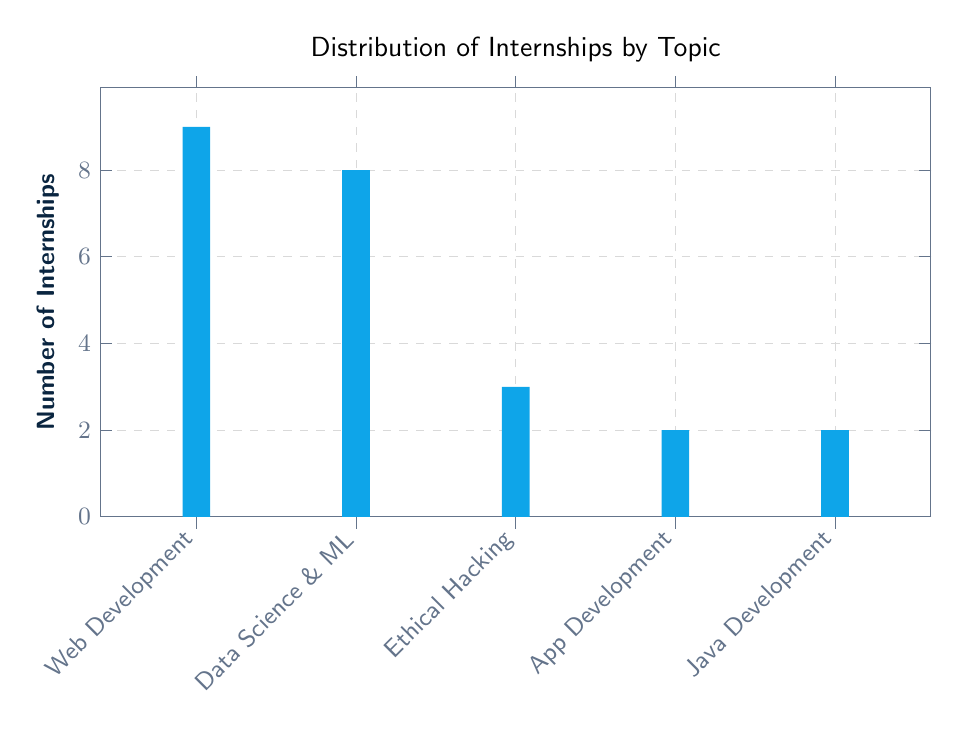
\begin{tikzpicture}
        \begin{axis}[
            institutional bar,
            title={Distribution of Internships by Topic},
            x tick label style={rotate=45, anchor=east},
            symbolic x coords={Web Development,Data Science \& ML,Ethical Hacking,App Development,Java Development},
            xtick=data,
            ylabel={Number of Internships},
            ymin=0,
            bar width=10pt,
            width=\textwidth, % Use full minipage width
            height=200pt,
        ]
        \addplot[fill=chart1, draw=none] coordinates {
            (Web Development,9) (Data Science \& ML,8) (Ethical Hacking,3) (App Development,2) (Java Development,2)
        };
        \end{axis}
        \end{tikzpicture}
    \end{minipage}%
    \hfill
    \begin{minipage}[t]{0.48\textwidth}
        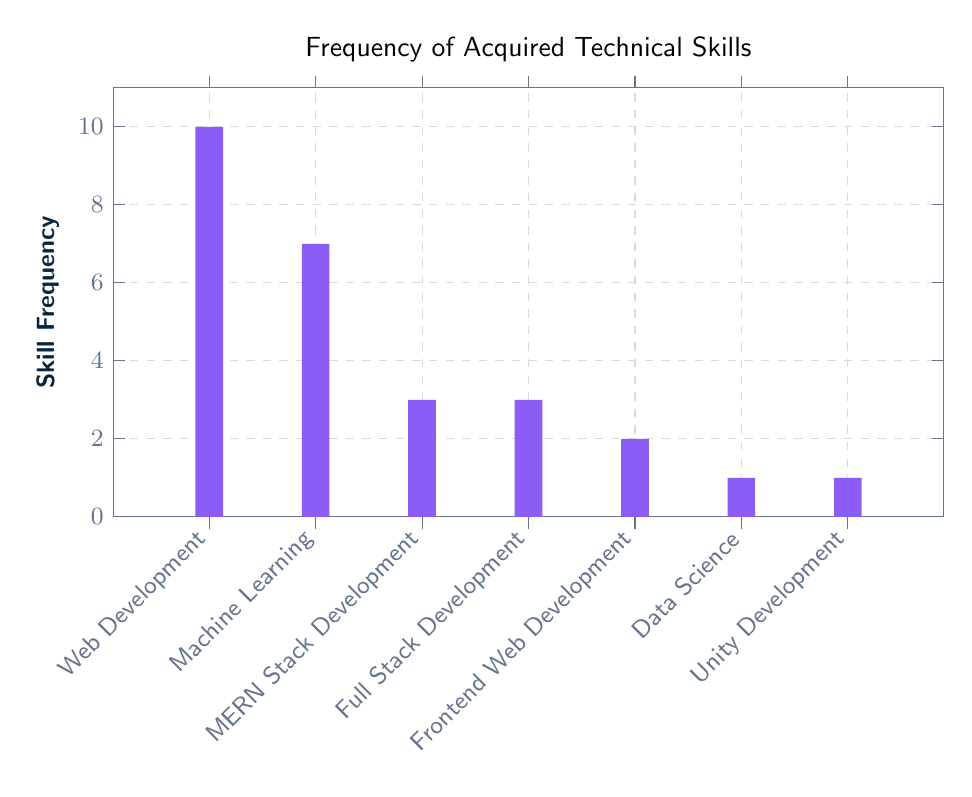
\begin{tikzpicture}
        \begin{axis}[
            institutional bar,
            title={Frequency of Acquired Technical Skills},
            x tick label style={rotate=45, anchor=east},
            symbolic x coords={Web Development,Machine Learning,MERN Stack Development,Full Stack Development,Frontend Web Development,Data Science,Unity Development},
            xtick=data,
            ylabel={Skill Frequency},
            ymin=0,
            bar width=10pt,
            width=\textwidth, % Use full minipage width
            height=200pt,
        ]
        \addplot[fill=chart2, draw=none] coordinates {
            (Web Development,10) (Machine Learning,7) (MERN Stack Development,3) (Full Stack Development,3) (Frontend Web Development,2) (Data Science,1) (Unity Development,1)
        };
        \end{axis}
        \end{tikzpicture}
    \end{minipage}
\end{card}

\vspace{0.5cm}

\begin{card}
    \subsection*{\textcolor{accent}{Detailed Internship Log (Sample)}}
    \vspace{0.3cm}
    \begin{longtable}{@{}p{0.03\textwidth}p{0.08\textwidth}p{0.1\textwidth}p{0.15\textwidth}p{0.07\textwidth}p{0.18\textwidth}p{0.2\textwidth}p{0.15\textwidth}@{}}
        \toprule
        \textbf{Sl.} & \textbf{Class Roll No.} & \textbf{Autonomy Roll No.} & \textbf{Student Name} & \textbf{Semester} & \textbf{Internship/ Training Provider} & \textbf{Internship/ Training Topic Name} & \textbf{Internship/ Training Duration} \\
        \midrule
        \endhead
        23 & 2154043 & 12621002012 & Aryan Gupta & 7th & RBW Solutions Private Limited & Backend Developer & 17th July, 2024 - 15th September, 2024 \\
        24 & 2154044 & 12621002058 & Yash Chokhani & 7th & InnoByte Services & Node.js Developer Intern & 25th June, 2024 - 25th July, 2024 \\
        25 & 2154045 & 12621002031 & Prabhat Kumar & 7th & OZIBOOK & Data Analyst Intern & 7th March, 2024 - 07th May, 2024 \\
        26 & 2154046 & 12621002051 & Srijan Kumar & 7th & Larsen \& Toubro (L\&T) & Digital and Data Analytics & 3rd June, 2024 - 25th July, 2024 \\
        27 & 2154047 & 12621002048 & Shiwang Raj & 7th & OASIS INFOBYTE & AICTE OIB-SIP internship in Java Development & 15th August, 2024 - 20th September, 2024 \\
        28 & 2154048 & 12621002039 & Rohit Kumar Gupta & 7th & Snackbae & Frontend Developer Intern & 28th May, 2024 - 27th July, 2024 \\
        \bottomrule
    \end{longtable}
\end{card}

\vspace{0.5cm}

\begin{card}
    \subsection*{\textcolor{accent}{Summary of Internships by Domain}}
    \vspace{0.3cm}
    \begin{longtable}{@{}p{0.5\textwidth}p{0.45\textwidth}@{}}
        \toprule
        \textbf{Internship/ Training Topic Name} & \textbf{Internship/ Training Duration} \\
        \midrule
        \endhead
        Software Engineering Virtual Experience (Establishing Financial Data Feeds, Frontend Web Development, Data Visualization with Perspective) & May, 2020 \\
        Android App Development & 1st May, 2020 to 12th June, 2020 (6 Weeks) \\
        Machine Learning with Python & 27th April, 2020 to 8th June, 2020 (6 Weeks) \\
        Data Science & 28th April, 2020 to 9th June, 2020 (6 Weeks) \\
        Data Science & 29th April, 2020 to 10th June, 2020 (6 Weeks) \\
        Data Science & 29th April, 2020 to 10th June, 2020 (6 Weeks) \\
        Ethical Hacking & 8 Weeks \\
        Machine Learning & 6th May, 2020 to 17th June, 2020 (6 Weeks) \\
        \bottomrule
    \end{longtable}
\end{card}

\clearpage

% ==================== SECTION: LEARNING OUTCOMES AND CHALLENGES ====================
\section*{\textcolor{accent}{Learning Outcomes and Challenges}}
\addcontentsline{toc}{section}{Learning Outcomes and Challenges}
{\large\textcolor{muted}{Analysis of practical experiences, learning, and challenges faced.}}

\vspace{0.5cm}

\begin{card}
    \subsection*{\textcolor{accent}{Learning Outcomes and Personal Development}}
    \vspace{0.3cm}
    The internship experiences provided a robust platform for the practical application of academic knowledge across a diverse array of IT domains. Students engaged in specialized roles such as Full Stack Development (e.g., Darzee, 6 months), Backend Development (e.g., RBW Solutions, 2 months; Intugine Technologies, 1 year), Frontend Development (e.g., Snackbae, 2 months), Data Analysis (e.g., OZIBOOK, 2 months), Machine Learning (e.g., multiple Internshala internships, 6-8 weeks; UPSKILL, 1.5 months), and Cyber Security (e.g., Ardent Computech, 1 month). This direct involvement in real-world projects, often spanning several months, facilitated a deeper understanding of how theoretical concepts in programming, data structures, algorithms, and system design translate into functional solutions. For instance, students in Node.js Developer Intern roles (e.g., InnoByte Services, 1 month) directly applied their knowledge of server-side programming and database interaction.

    The internships significantly contributed to improved coding proficiency and an understanding of industry workflows. Students undertaking roles in Web Development (e.g., Octanet, 2 months; Internshala, 6-8 weeks), Android App Development (e.g., EUPHORIA GENX, 2 months), and Java Development (e.g., OASIS INFOBYTE, 1 month) gained hands-on experience with various programming languages and frameworks. Exposure to companies ranging from startups like InnoByte Services and Snackbae to established corporations such as Larsen \& Toubro (L\&T), Tata Steel Limited, and JPMORGAN CHASE \& CO. provided insights into diverse organizational structures, project management methodologies, and professional development cycles. This exposure was crucial for understanding version control, collaborative coding practices, and adherence to industry standards, which are integral to successful software development.

    Beyond technical skills, the internships fostered substantial personal growth, confidence building, and career path clarification. Engaging in roles that required problem-solving, independent research, and collaboration within a professional setting naturally enhanced self-reliance and communication skills. The breadth of topics, from ``Ethical Hacking and Cyber Security'' to ``Cloud-Storage Enabled Data Analytics for IoT Systems in Smart Agriculture'' and ``Vendor Invoice Management on eVIDIT,'' allowed students to explore various facets of the IT industry. This exploration, coupled with the successful completion of projects, contributed to increased confidence in their abilities and provided valuable clarity regarding their preferred career trajectories and areas of specialization post-graduation.
\end{card}

\vspace{0.5cm}

\begin{card}
    \subsection*{\textcolor{accent}{Challenges Faced and Solutions}}
    \vspace{0.3cm}
    The diverse array of technical internships undertaken by students, spanning areas such as Full Stack Development (e.g., Darzee, Breakview Studios), Backend Development (e.g., RBW Solutions, Intugine Technologies), Frontend Development (e.g., Snackbae, Bytelearn), Data Science, Machine Learning, and AI (e.g., OZIBOOK, Internshala, UPSKILL, Ardent AI), inherently presented significant technical challenges. Students frequently encountered steep learning curves, particularly when adapting to new programming languages, frameworks (e.g., Node.js, ReactJS), or complex domain-specific tools within durations ranging from 1 month to 6 months. For instance, a student undertaking a 6-week Machine Learning internship (e.g., Internshala) would face intense pressure to rapidly acquire and apply advanced analytical skills, while a Full Stack Developer intern (e.g., Darzee, 6 months) would navigate the complexities of integrating multiple technologies across an extended project lifecycle. The varied project requirements, from developing note-making and chatting applications (e.g., Euphoria Genx) to managing vendor invoices on eVIDIT (e.g., Indian Oil Corporation Limited), demanded not only technical proficiency but also a rapid understanding of specific business contexts and operational workflows.

    To navigate these obstacles, students employed a range of proactive strategies. A primary approach involved intensive self-directed learning, leveraging online documentation, tutorials, and internal company resources to bridge knowledge gaps quickly. For instance, interns in specialized fields like Cloud-Storage Enabled Data Analytics for IoT Systems (e.g., IIT Roorkee) or Ethical Hacking (e.g., Ardent Computech) would have necessitated continuous research and practical application to master complex concepts. Furthermore, active engagement with mentors and team members was crucial for clarifying project requirements, understanding best practices, and troubleshooting technical issues. The collaborative nature of many development roles, such as SDE Internships (e.g., Revirt Space, Breakview Studios), underscored the importance of effective communication and teamwork in resolving complex problems and ensuring project progression.

    The experience of overcoming these challenges fostered significant professional development. Students cultivated enhanced problem-solving abilities, learning to systematically diagnose and resolve technical impediments under real-world constraints. The necessity of rapidly acquiring new skills and adapting to diverse project environments, from web application development (e.g., Tata Steel Limited) to data analytics (e.g., L\&T Digital and Data Analytics), instilled a strong sense of adaptability and resilience. These internships served as critical platforms for translating theoretical knowledge into practical application, reinforcing the importance of continuous learning and iterative development in the dynamic IT landscape. The exposure to professional workflows and industry standards also refined students' time management and project execution skills, preparing them for future roles in the technology sector.
\end{card}

\vspace{0.5cm}

\begin{card}
    \subsection*{\textcolor{accent}{Internship Duration Breakdown}}
    \vspace{0.3cm}
    \begin{center}
        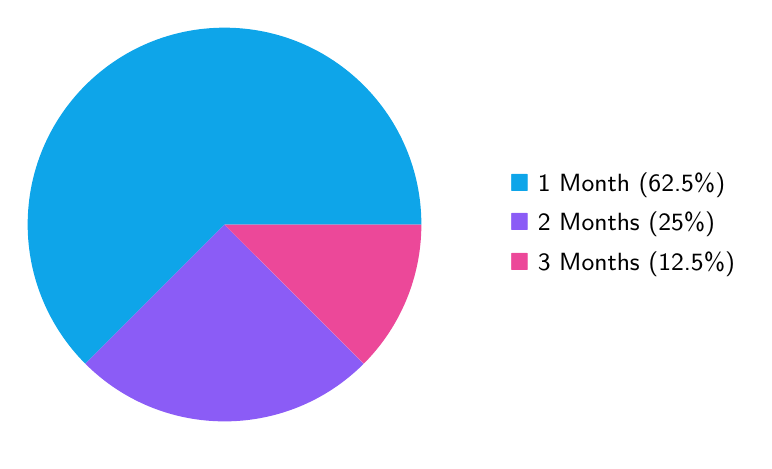
\begin{tikzpicture}
        \coordinate (center) at (0,0);
        \def\radius{2.5cm}
        \pgfmathsetmacro{\totaldata}{5+2+1} % Sum of all data points (5+2+1 = 8)
        
        % Data: 1 Month (5), 2 Months (2), 3 Months (1)
        % Percentages: 5/8=62.5%, 2/8=25%, 1/8=12.5%
        
        \pgfmathsetmacro{\angleA}{5/(\totaldata)*360} % 1 Month
        \pgfmathsetmacro{\angleB}{2/(\totaldata)*360} % 2 Months
        \pgfmathsetmacro{\angleC}{1/(\totaldata)*360} % 3 Months

        \fill[chart1] (center) -- (0:\radius) arc (0:\angleA:\radius) -- cycle;
        \fill[chart2] (center) -- (\angleA:\radius) arc (\angleA:\angleA+\angleB:\radius) -- cycle;
        \fill[chart3] (center) -- (\angleA+\angleB:\radius) arc (\angleA+\angleB:\angleA+\angleB+\angleC:\radius) -- cycle;

        \node[anchor=west, font=\small] at (3.5, 0.5) {\textcolor{chart1}{$\blacksquare$} 1 Month (62.5\%)};
        \node[anchor=west, font=\small] at (3.5, 0) {\textcolor{chart2}{$\blacksquare$} 2 Months (25\%)};
        \node[anchor=west, font=\small] at (3.5, -0.5) {\textcolor{chart3}{$\blacksquare$} 3 Months (12.5\%)};
        \end{tikzpicture}
    \end{center}
\end{card}

\vspace{0.5cm}

\begin{card}
    \subsection*{\textcolor{accent}{Comparison of Internship Types (Industry vs. Online)}}
    \vspace{0.3cm}
    \begin{longtable}{@{}p{0.25\textwidth}p{0.4\textwidth}p{0.3\textwidth}@{}}
        \toprule
        \textbf{Internship/ Training Provider} & \textbf{Internship/ Training Topic Name} & \textbf{Internship/ Training Duration} \\
        \midrule
        \endhead
        Ardent & Network Penetration Testing using METASPLOITABLE & 20/07/2022-25/08/2022 \\
        Internshala & Web Development & Eight Weeks \\
        Internshala & Web Development & Eight Weeks \\
        Varzeo Internship Program & Web Development & 20/07/2022-20/09/2022 \\
        Bambus Group Internship Program & (Junior Developer Trainee) on DEV OPS & 01/08/2022-31/10/2022 \\
        Internshala & REACT JS & Six Weeks \\
        Internshala & Machine Learning & Six Weeks \\
        Internshala & Machine Learning & Six Weeks \\
        Bytelearn & Frontend Developer Intern & July, 2022 - Nov, 2022 \\
        \bottomrule
    \end{longtable}
\end{card}

\clearpage

% ==================== SECTION: RECOMMENDATIONS AND FUTURE OUTLOOK ====================
\section*{\textcolor{accent}{Recommendations and Future Outlook}}
\addcontentsline{toc}{section}{Recommendations and Future Outlook}
{\large\textcolor{muted}{Strategic recommendations for enhancing future internship programs.}}

\vspace{0.5cm}

\begin{card}
    \subsection*{\textcolor{accent}{Recommendations for Future Internships}}
    \vspace{0.3cm}
    To enhance the internship program for future students, a critical review of internship durations and types of engagement is recommended. While a significant number of students undertook shorter programs, such as the numerous 6-week and 8-week internships facilitated by Internshala across various domains like Web Development, Machine Learning, and Data Science, longer durations appear to correlate with more specialized roles. For instance, Darzee offered a 6-month Full Stack Developer role, Intugine Technologies provided a nearly year-long Backend Development opportunity, and Bytelearn and Revirt Space offered 5-month and 4-month SDE Internships, respectively. Future program improvements should encourage students to pursue these extended engagements, which likely offer deeper immersion and more substantial project contributions. Furthermore, the program should continue to support the diverse range of technical topics observed, including Backend, Frontend, Node.js, Java, Python, AI, Machine Learning, Data Analytics, Ethical Hacking, and Cyber Security, ensuring a broad skill development pathway. The inclusion of structured programs, such as the AICTE OIB-SIP internship in Java Development, also presents a valuable model for future offerings.

    Collaboration with industry partners can be significantly enhanced by focusing on the quality and duration of placements. The current report highlights a wide array of partners, from startups like InnoByte Services and Snackbae to established corporations such as Larsen \& Toubro (L\&T), Indian Oil Corporation Limited, Tata Steel Limited, and global entities like JPMORGAN CHASE \& CO. and Accenture Nordic. To deepen these relationships, the department should actively seek to formalize partnerships that facilitate longer-term internships, similar to the 6-month engagement with Darzee or the nearly year-long stint at Intugine Technologies. These extended periods allow for more meaningful project involvement and foster stronger ties between the academic institution and industry. Additionally, exploring and expanding opportunities for virtual experience programs, as offered by JPMORGAN CHASE \& CO. and Accenture Nordic, can broaden access to a wider range of companies and specialized roles, complementing traditional in-person placements.

    For students preparing for future internships, the current experiences underscore the importance of developing robust technical skills in high-demand areas. The prevalence of roles in Web Development (including Full Stack, Frontend, Backend, Node.js, and ReactJS), Machine Learning, Data Science, AI, Java Development, and Python indicates these are critical competencies. Students should prioritize hands-on project work in these domains to build a strong portfolio. Furthermore, based on the varied durations observed, students are advised to actively seek internships that extend beyond the typical 6-8 week period, aiming for opportunities of two months or more. Longer engagements, such as the 4-5 month roles at Bytelearn and Revirt Space, or the 6-month position at Darzee, provide more comprehensive learning and practical application of skills. Finally, students should diversify their search strategies, exploring opportunities not only through online platforms but also directly with companies, academic institutions like IIT Roorkee, and through structured programs like AICTE OIB-SIP, to maximize their exposure to diverse industry environments and challenges.
\end{card}

\vspace{0.5cm}

\begin{card}
    \subsection*{\textcolor{accent}{Top Internship Providers}}
    \vspace{0.3cm}
    \begin{center}
        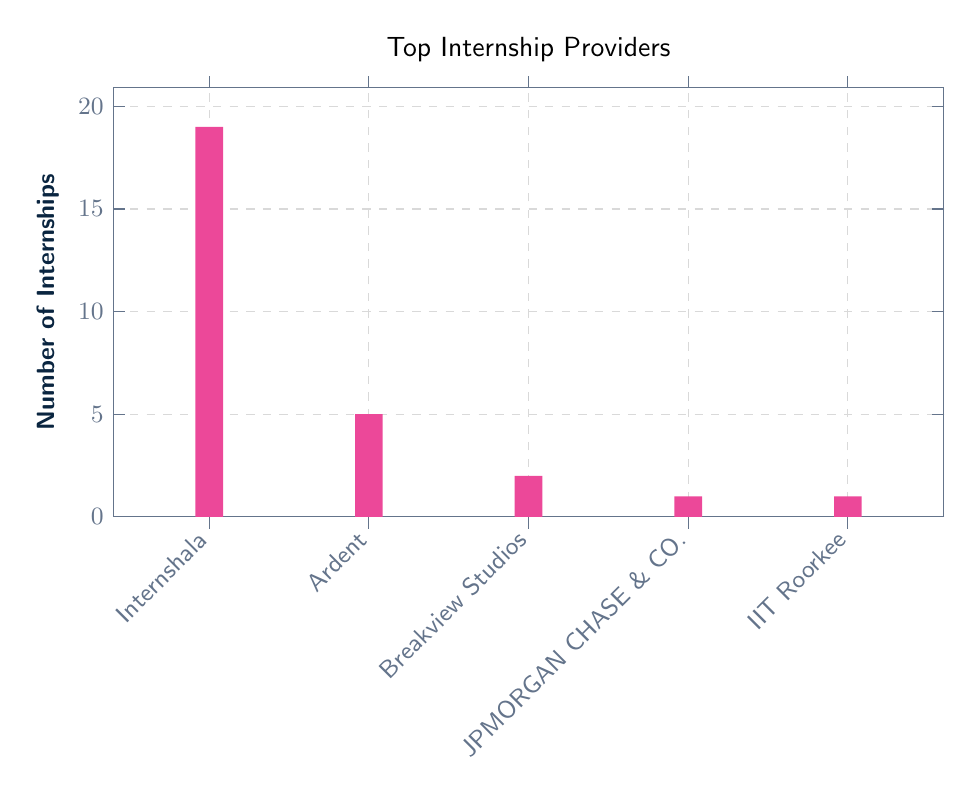
\begin{tikzpicture}
        \begin{axis}[
            institutional bar,
            title={Top Internship Providers},
            x tick label style={rotate=45, anchor=east},
            symbolic x coords={Internshala,Ardent,Breakview Studios,JPMORGAN CHASE \& CO.,IIT Roorkee},
            xtick=data,
            ylabel={Number of Internships},
            ymin=0,
            bar width=10pt,
            width=\textwidth, % Use full minipage width
            height=200pt,
        ]
        \addplot[fill=chart3, draw=none] coordinates {
            (Internshala,19) (Ardent,5) (Breakview Studios,2) (JPMORGAN CHASE \& CO.,1) (IIT Roorkee,1)
        };
        \end{axis}
        \end{tikzpicture}
    \end{center}
\end{card}

\end{document}